% -*- root: ../../DAT2-A423_Project_Report.tex -*-
\clearpage
\section{Overview of ``A Graph-Theoretic Approach to Steganography''}
\label{sec:graphtheory}
{\footnotesize This section is based on the article by Hetzl and Mutzel\citep{hetzl_2005} and Olav Geil's lecture on the article.}

\subsection{Goal of the Method}
Methods such as LSB can be used to embed a lot of information in images. 
With the implementation described in section \ref{sec:lsb-implementation} we were able to embed six bits of information in each pixel in a true-colour bitmap. 
The downside of this method, as described in section \ref{steganalysis}, is that it is very easy to detect because it forcibly changes a lot pixel in the image. 

The goal of the following method is to change as little as possible in the image, while still being able to embed its message.

In the following examples, we start out with the image seen on figure \ref{fig:startingImage}.
The message to be concealed in the image is the binary string $10100110011010$.

\begin{figure}[h!]
	\centering
	
\includegraphics[width=.4\textwidth, frame]{figures/pixelgrid.png}
	\caption{Grey-scale cover image}
	\label{fig:startingImage}
\end{figure}

\subsection{Terminology}
First we define the function $v$ as $ v_m: \mathds{Z} \Rightarrow \{0,1,2,\ldots,m-1\} $ such that $ v_m(s) = s \mod m $. 
Furthermore we have the message, $e$ a list of $n$ elements, to encode in the image: $e = \{ e_0, e_1, e_2, \ldots, e_n \}$, where $\forall i\left( e_i < m \right)$. 
Because all entries in the message list to be encoded must be less than $m$, $m$ defines the number of actual bits can be transferred in each pair of pixels. With $m = 2$ the only two possible values are $0$ and $1$, which means that only one bit can be embedded as one entry in the message vector.
By choosing $m = 4$, the possible values are $0$, $1$, $2$ and $3$, or $00_2$, $01_2$, $10_2$ and $11_2$.
Practically this means that we can embed two bits in every entry in the message vector. 

The $\oplus_m$ operator is used for computing sums modulo $m$.
In other words, the operator describes the calculation $x \oplus_m y = v_m(x + y) = (x + y) \mod m$.  

In the following example we will use $m = 4$, as this allows 2 bits to be used for each entry in the message vector.
Our message vector is found by splitting the binary string into pairs of two bits, which then makes it $e = [10 \, 10 \, 01 \, 10 \, 01 \, 10 \, 10]$. 

\subsection{Method Described in Article}
A grey-scale image can be viewed as a list of pixels $p = \{ p_0, p_1, p_2, \ldots, p_n \}$, where $\forall i\left( 0 \leq p_i \leq 255 \right)$. 
These pixels are then ordered into consecutive pairs of two.
Because we embed one entry from the message vector into each pair of pixels, an $m$ value of 4, means that we embed two bit per two pixels, meaning the message vector can have the same dimension as the amount of pixels in the image. 
Were we to choose $m = 2$, only half of this message could fit in the same image.
The $\oplus_m$ operator is then used on each individual pair, and compared to the message which is to be encoded.
If the resulting remainder equals the wanted message, these pixels are a \textit{perfect pair}.
If not, they need to be changed by either switching two pixels around, or changing one of the values.
In this method we want to avoid changing the values directly.
Instead, we find all pairs of pixels that could be interchanged and result in perfect pairs.
In table \ref{PairOrdering} this method is applied to the grey-scale image on figure \ref{fig:startingImage} with 14 pixels, and the message vector with seven entries. 

\begin{table}[h]
\centering
\caption{Process of finding pixels in need of changing or switching}
\label{PairOrdering}
\resizebox{\textwidth}{!}{%
\begin{tabular}{|c|c|c|c|c|c|c|c|c|c|c|c|c|c|c|}
\hline
Pixel & 1 & 2 & 3 & 4 & 5 & 6 & 7 & 8 & 9 & 10 & 11 & 12 & 13 & 14 \\ \hline
Value & 106 & 102 & 103 & 100 & 101 & 101 & 200 & 255 & 100 & 125 & 103 & 254 & 104 & 100 \\ \hline
$\oplus_4$ & \multicolumn{2}{c|}{0} & \multicolumn{2}{c|}{3} & \multicolumn{2}{c|}{2} & \multicolumn{2}{c|}{3} & \multicolumn{2}{c|}{1} & \multicolumn{2}{c|}{1} & \multicolumn{2}{c|}{0} \\ \hline
Message & \multicolumn{2}{c|}{2} & \multicolumn{2}{c|}{2} & \multicolumn{2}{c|}{1} & \multicolumn{2}{c|}{2} & \multicolumn{2}{c|}{1} & \multicolumn{2}{c|}{2} & \multicolumn{2}{c|}{2} \\ \hline
 & \multicolumn{2}{c|}{$\neq$} & \multicolumn{2}{c|}{$\neq$} & \multicolumn{2}{c|}{$\neq$} & \multicolumn{2}{c|}{$\neq$} & \multicolumn{2}{c|}{=} & \multicolumn{2}{c|}{$\neq$} & \multicolumn{2}{c|}{$\neq$} \\ \hline
Needed values & \multicolumn{2}{c|}{\begin{tabular}[c]{@{}c@{}}<104,100>\\ <108,104>\end{tabular}} & \multicolumn{2}{c|}{\begin{tabular}[c]{@{}c@{}}<102,99>\\ <106,103>\end{tabular}} & \multicolumn{2}{c|}{\begin{tabular}[c]{@{}c@{}}<100,100>\\ <104,104>\end{tabular}} & \multicolumn{2}{c|}{\begin{tabular}[c]{@{}c@{}}<199,254>\\ <203,002>\end{tabular}} & \multicolumn{2}{c|}{} & \multicolumn{2}{c|}{\begin{tabular}[c]{@{}c@{}}<100,251>\\ <104,255>\end{tabular}} & \multicolumn{2}{c|}{\begin{tabular}[c]{@{}c@{}}<102,98>\\ <106,102>\end{tabular}} \\ \hline
\end{tabular}%
}
\end{table}

From the table we can see that switching the following pixels would make more pairs correct $(4 \leftrightarrow 11)$, $(8\leftrightarrow 12)$, $(2\leftrightarrow 13)$ and $(1 \leftrightarrow 13)$.

As a graph, these switches can be represented as on figure \ref{fig:graph}. 
Each vertex represents a pair of pixels, where at least one of the pixels can be changed. The edges describe a switch between two pixels. 
This graph can then be used to determine which switches to make.
Every time a switch is made, all other edges touching the two vertices where pixels are changed, are removed.
This graph can be used to determine which switches are the best, by introducing edge weight, describing how much of a visual change, a switch would result in.

\begin{figure}[h!]
\centering
\begin {tikzpicture}[-latex ,auto ,node distance =0.65 cm and 0.65cm ,on grid ,
semithick ,
state/.style ={ circle ,top color =white ,
draw , text=black , minimum width =0.3111111111111111 cm},
state2/.style ={ circle ,color =white ,
draw , text=black, opacity=0.0 , minimum width =.3 cm}]
\node[state] (A0) {(1,2)};
\node[state2] (A1) [right =of A0] {};
\node[state2] (A2) [right =of A1] {};
\node[state2] (A3) [right =of A2] {};
\node[state2] (A4) [right =of A3] {};
\node[state2] (A5) [right =of A4] {};
\node[state2] (A6) [right =of A5] {};
\node[state2] (A7) [right =of A6] {};
\node[state2] (A8) [right =of A7] {};
\node[state2] (A9) [right =of A8] {};
\node[state2] (A10) [below =of A9] {};
\node[state2] (A11) [below =of A10] {};
\node[state] (A12) [below =of A11] {(3,4)};
\node[state2] (A13) [left =of A12] {};
\node[state2] (A14) [left =of A13] {};
\node[state2] (A15) [left =of A14] {};
\node[state2] (A16) [below =of A15] {};
\node[state2] (A17) [below =of A16] {};
\node[state] (A18) [below =of A17] {(7,8)};
\node[state2] (A19) [right =of A18] {};
\node[state2] (A20) [right =of A19] {};
\node[state] (A21) [right =of A20] {(11,12)};
\node[state2] (A22) [left =of A21] {};
\node[state2] (A23) [left =of A22] {};
\node[state2] (A24) [left =of A23] {};
\node[state2] (A25) [left =of A24] {};
\node[state2] (A26) [left =of A25] {};
\node[state] (A27) [left =of A26] {(13,14)};
\path[-] (A12) edge node[] {$4 \leftrightarrow 11$}(A21);
\path[-] (A18) edge node[right=-.6cm,above=.6cm] {$8\leftrightarrow 12$}(A21);
\path[-] (A0) edge [bend right =-45] node[] {$2\leftrightarrow 13$}(A27);
\path[-] (A0) edge [bend right =45] node[] {$1 \leftrightarrow 13$}(A27);
\end{tikzpicture}
\caption{Graph containing the possible switches}
\label{fig:graph}
\end{figure}

Let us say that the switches $2\leftrightarrow 13$ and $4\leftrightarrow 11$ are chosen.
The pixels after these switches are shown in table \ref{tab:pixelsSwitched}.
We would still need to correct the pairs (5,6) and (7,8).
There is no switch that allows us to correct these values, so instead the actual values are forcibly changed and by doing so, change the image ever so slightly. 

\begin{table}[h]
\caption{Pixels after switching}
\label{tab:pixelsSwitched}
\centering
\resizebox{\textwidth}{!}{%
\begin{tabular}{|c|c|c|c|c|c|c|c|c|c|c|c|c|c|c|}
\hline
Pixels & $p_1$ & $p_2$ & $p_3$ & $p_4$ & $p_5$ & $p_6$ & $p_7$ & $p_8$ & $p_9$ & $p_{10}$ & $p_{11}$ & $p_{12}$ & $p_{13}$ & $p_{14}$ \\ \hline
Value & 106 & 104 & 103 & 103 & 101 & 101 & 200 & 255 & 100 & 125 & 100 & 254 & 102 & 100 \\ \hline
$\oplus_4$ & \multicolumn{2}{c|}{2} & \multicolumn{2}{c|}{2} & \multicolumn{2}{c|}{2} & \multicolumn{2}{c|}{3} & \multicolumn{2}{c|}{1} & \multicolumn{2}{c|}{2} & \multicolumn{2}{c|}{2} \\ \hline
Message & \multicolumn{2}{c|}{2} & \multicolumn{2}{c|}{2} & \multicolumn{2}{c|}{1} & \multicolumn{2}{c|}{2} & \multicolumn{2}{c|}{1} & \multicolumn{2}{c|}{2} & \multicolumn{2}{c|}{2} \\ \hline
 & \multicolumn{2}{c|}{=} & \multicolumn{2}{c|}{=} & \multicolumn{2}{c|}{$\neq$} & \multicolumn{2}{c|}{$\neq$} & \multicolumn{2}{c|}{=} & \multicolumn{2}{c|}{=} & \multicolumn{2}{c|}{=} \\ \hline
Needed values & \multicolumn{2}{c|}{} & \multicolumn{2}{c|}{} & \multicolumn{2}{c|}{\begin{tabular}[c]{@{}c@{}}<100,100>\\ <104,104>\end{tabular}} & \multicolumn{2}{c|}{\begin{tabular}[c]{@{}c@{}}<199,254>\\ <203,003>\end{tabular}} & \multicolumn{2}{c|}{} & \multicolumn{2}{c|}{} & \multicolumn{2}{c|}{} \\ \hline
\end{tabular}%
}
\end{table}


The image obtained after these switches and changes are the one shown on figure \ref{fig:endingImageComp} next to the original image shown on figure \ref{fig:startingImageComp}.


\begin{figure}[h!]
    \centering
    \begin{subfigure}[b]{0.45\textwidth}
        
\includegraphics[width=\textwidth, frame]{figures/pixelgrid.png}
		\caption{Grey-scale cover image}
		\label{fig:startingImageComp}
    \end{subfigure}
    ~ %add desired spacing between images, e. g. ~, \quad, \qquad, \hfill etc. 
      %(or a blank line to force the subfigure onto a new line)
    \begin{subfigure}[b]{0.45\textwidth}
        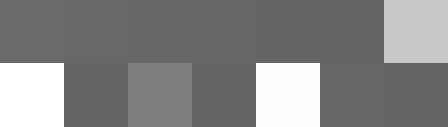
\includegraphics[width=\textwidth, frame]{figures/pixelgrid2.png}
		\caption{Grey-scale stego image}
		\label{fig:endingImageComp}
    \end{subfigure}
    \caption{Comparison of the image before (\ref{fig:startingImageComp}) and after (\ref{fig:endingImageComp}) the changes have been made.}\label{fig:pixelGrids}
\end{figure}

By doing these switches, we minimize the need to alter the pixels in the image.
With methods such as LSB it is rarely the case that pixels do not need to be altered.
This method is much more resistant to statistical analysis, such as the colour histograms described in section \ref{steganalysis}.

When the message is to be extracted from the image, the same method of grouping pixels into pairs are applied.
Now, instead of trying to find pairs to be switched, the value obtained after using the $\oplus_m$ operation are the values embedded in the image.
These values can then be grouped into a vector, which is a copy of the original message vector.